\documentclass[a4paper]{article}

\usepackage[english]{babel}
\usepackage[utf8]{inputenc}
\usepackage{amsmath}
\usepackage{graphicx}
\usepackage{natbib}
\usepackage{filecontents}
\usepackage{url}
\usepackage{hyperref}
\usepackage[paper=a4paper]{geometry}

\newgeometry{top=1in,right=1.5in,left=1.5in}

\title{Sentiment analysis with linear regression and LSTM}

\author{Language Processing II exam \\ Jens Egholm Pedersen \\ \texttt{xtp778@sc.ku.dk}}

\date{\today}

\begin{document}
\begin{titlepage}
\maketitle

\tableofcontents
\end{titlepage}

\newgeometry{top=1in,bottom=1in,right=1.5in,left=1.5in}
\pagebreak

\section{Introduction}
\label{sec:introduction}
Due to the enormous rise in accessible data and processing capabilities,
computers have been moving from the restricted formalized domain of
mathematics and computability, and into the more complex and seemingly
chaotic domain of natural language \citep{NILSSON2009, Jurafsky2000}. Automating
understanding of natural language has a wide range of helpful applications,
from translation to recommender systems to generic personal assistants
\citep{COX2005, BKL2009}.

As a part of this development, sentiment analysis has been attracting increased
attention \citep{BKL2009, Jurafsky2000}. Along with modern deep learning
techniques, sentiment prediction models have reached a higher precision
than ever before \citep{Jurafsky2000, Schmidhuber2015}.
Especially long short-term memory (LSTM) networks have shown staggering results
within the field \citep{Schmidhuber2015}.

In the present paper a corpus of movie reviews presented by \cite{PangLee2005}
is applied to four sentiment analysis models.
Two of the models build on a simple linear regression model, while the other
two employ modern LSTM techniques. The data is preprocessed using natural
language processing tools and injected in the models with 4-fold cross
validation.

\section{Background}
\label{sec:background}
This section illuminates the theory and background for language processing
and basic methodology for processing text.
Sentiment analysis as a fundamental concept for this setting will be introduced
second, followed by fundamental statistical metrics. Lastly,
recurrent neural networks will be introduced before moving on to the data
generation.

\subsection{Language processing}
Following the revolutionizing formalizations of grammar by \cite{Chomsky2002},
first written in 1957, much work was put into working with the computability
of language \citep{Jurafsky2000}. In the beginning of the 21st century,
the previous work converged with the statistical machine learning community,
giving rise to supervised, semi-supervised and even unsupervised models
of language understanding and translation \citep{Jurafsky2000}.

There are several approaches to language processing, but it is common
to deconstruct text into its constituents and assign meaning
to each piece, with the hope that the disassembly gives additional meaning
that can aggregate to an understanding of the text as a whole, when the pieces
are put back together \citep{Jurafsky2000}.
\textit{Constituents} can range from morphemes to words to whole sentences in
this context. This process is referred to as feature extraction due to the
enrichment of the text with meta-data.

A fundamental method for feature extraction is to construct a probabilistic
model by simply joining items (ranging from phonemes to word pairs) together
in pairs of one, two or more, called \textit{n}-grams \citep{Jurafsky2000}.
The advantage of this approach focuses on speed and the simple, yet efficient,
probabilities in for instance word pairs which can be applied to predict
likelihood of future occurrences \citep{Jurafsky2000}.

Term frequency, inverse document frequency (tf-idf) is another relevant feature
that describes the relevance of an item, weighted against the number of
times it appears in other documents \citep{Jurafsky2000} (see figure \ref{fig:tfidf}).
Tf-idf favors words that are used heavily in a
single document (assumed to be important) while diminishing the importance of
words that often occur in other documents, and is a heavily used metric \citep{Jurafsky2000}.

\begin{figure}
\[tf-idf = Nw \cdot log(\frac{N}{k})\]
\caption{Formula for tf-idf.}
\label{fig:tfidf}
\end{figure}

\subsubsection{Sentiment analysis}
Another popular approach for disassembling text
called part of speech-tagging (POS tagging), assigns grammatical categories
to each word and attempt to build a linguistic model that can be understood by
a machine \citep{Jurafsky2000}. This works well for information retrieval,
where objective truths can be extracted\footnote{Such as the objective statements about an object in the
sentence "\textit{The cat likes tuna fish}".}, but fails
to capture the complexity and emotional variety of sentences that appear
outside the grammar, such as emotions and opinions\footnote{One example is a heavily sarcastic sentence like
"\textit{I'd really truly love going out in this weather!}". For POS-tagging
sarcasm is difficult to capture because it is not implicitly encoded in the
grammatical categories.} \citep{Jurafsky2000}.
\label{text:irony}

Sentiment analysis focuses on extracting information about the emotions or
opinions of a text \citep{PangLee2008}.
Defining the word \textit{sentiment} is not a simple task, and has been
scrutinized extensively \citep{Jurafsky2000, PangLee2008}.
A much used approach was introduced by \cite{Ekman92} where he devised six
basic emotions, which could be conveniently operationalized by computers.
Since the dataset for this paper revolves around opinions in a single dimension,
\textit{sentiment} will in this paper simply refer to a subjective experience,
discretized to a number (see section \ref{sec:dataset}).

\subsection{Linear regression}
Linear regression is a mathematical function that describes how the mean of the
output changes with the value of the input \citep{Agresti2008}. The model is
appropriate when a linear correlation between the input and output can be
assumed, so an increase in the input results in a linear in- or decrease in
the output, represented by a straight line in a 2-dimensional coordinate system
\citep{Agresti2008}.

\subsubsection{Error reporting}
The predictions made by a linear regression model ($y$) does not always fit
the actual values ($ŷ$). To describe this error and to give indicators on the
quality of the model, the mean absolute error (MAE) and root mean squared
error (RMSE) is introduced \citep{Agresti2008, Chai2014}.

MAE in figure \ref{fig:mae} describes the mean of the absolute error values.
If a model has an MAE of 1, the average distance to the actual value from the
predicted value is 1. The bigger the mean error value, the worse the model is.

\begin{figure}
\[MAE = \frac{\Sigma |e|}{n}, e = y - ŷ\]
\caption{Mean absolute error (MAE).}
\label{fig:mae}
\end{figure}

However, this figure does not capture the error distribution of the model
\citep{Chai2014}. If
a Gaussian distribution is assumed for the errors, it is important to know
the standard distribution to indicate \textit{how} consistently wrong the model
is \citep{Agresti2008}. The root mean square error measures the standard
deviation in the sample of the errors, making it a good description for the
model accuracy, compared to other models \citep{Agresti2008, Chai2014}.

\begin{figure}
\[ RMSE = \sqrt{\frac{\Sigma (e)^{2}}{n - 2}}, e = y - ŷ \]
\caption{Root mean square error (RMSE).}
\label{fig:rmse}
\end{figure}

Each metric should not stand alone however, and MAE and RMSE are typically
reported together \citep{Chai2014}.

\subsection{Neural networks}
Inspired by the biological brain, models for neural networks have been applied
in computer science since the 1950s, and have become integral part of machine
learning \citep{NILSSON2009, Russell2009}.
Neurons are essentially functions that operate on some input and respond with
some output \citep{Russell2009}. The inputs for a neuron are weighted to give
different input channels - or input dimensions - varying significance. These
weighted inputs arrive to an activation function that decides whether the
neuron should ‘fire’ or not \citep{NILSSON2009}. Sigmoid or hyperbolic tangent
are popular
activation functions for numerical predictions because of their steep logistic
properties while retaining differentiability. Neural networks excel in their
adaptability and have long been applied to the field of language processing
\citep{Jurafsky2000}.

Simple neural networks can be stacked in layers, where each neuron will assign
weights to the input, to determine its significance for the activation function
\citep{NILSSON2009}. By tuning the weights of the neurons, such groupings can
learn to fire on certain input patterns \citep{Russell2009}. However,
this structure have proved brittle and difficult to train because the
neurons do not retain their weights for long \citep{NILSSON2009, Russell2009}.
\cite{Rumelhart1988} suggested a method to avoid this instability by adjusting
the weights of the neurons in retrospect with a method called back-propagation
\citep{Rumelhart1988, NILSSON2009}. This optimization is
operationalized by a function that can describe the \textit{loss} of effiency
in a network, and then adjust the weights correspondingly using gradient
descent \citep{Russell2009}.

\subsubsection{Long short-term memory networks}
Back-propagating networks with a high complexity in layers and neurons have
shown to be hard to optimize above a certain point, because the gradient
descent algorithm are inefficient at escaping local extrema in a high-dimensional
space \citep{Russell2009}. Recurrence have been used to counter this problem,
by conserving \emdash or returning to \emdash previous, optimal values
\citep{Schmidhuber2015, Russell2009}. \cite{Hochreiter1997} suggested a certain
type of memory-retaining networks that is able to balance between both
storing previous optimal state, while also forgetting context when new and
different input arrives \citep{Hochreiter1997, Schmidhuber2015}.
They dubbed the model long short-term memory (LSTM) networks, to capture both
properties \citep{Hochreiter1997}.

\begin{figure}
  \centering
  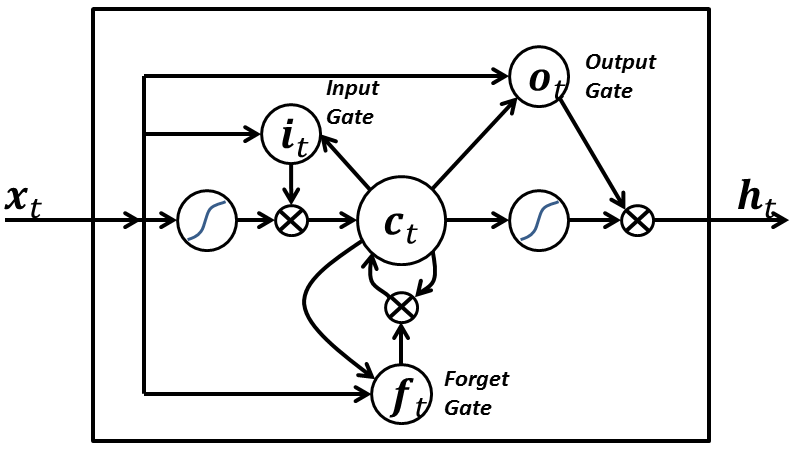
\includegraphics[width=0.8\textwidth]{lstm.png}
  \caption{A \textit{peephole} LSTM unit with three gates (input, output and forget).}
  \label{fig:lstm}
\end{figure}

The LSTM model seen in figure \ref{fig:lstm} builds on the idea of a more
complex neuronal unit, with several \textit{gates}, collaborating to give
the LSTM the desired property \citep{Gers2001}. A traditional unit contains
three gates: an "input" gate that controls the degree with which new information
should influence the current memory state, a "forget" gate that decides whether
a value should be retained and an output gate that decides how much influence
the memory should have on the activation of the unit \citep{Hochreiter1997, Gers2001}.
There are a plentitude of other architectures, but for this paper, the LSTM
model shown in figure \ref{fig:lstm} is used \citep{Gers2001}.

\subsubsection{Optimization and regularization}
Recurrent neural networks are typically trained with a continuously applied
loss function and gradient descent for weight correction \citep{Russell2009,
Hochreiter1997, Schmidhuber2015}. Stochastic gradient descent and resilient
back-propagation are two common approaches, which have proved efficient
\citep{Russell2009, NILSSON2009}. This paper applies a third method, based on
the RMSE algorithm in figure \ref{fig:rmse}, called root mean square propagation
(RMSprop), which preserves the stochastic properties while controlling
for previous errors in the network \citep{Tieleman2012}.

LSTMs and machine learning models in general can overfit to the data
they are trained on, loosing their ability to predict data outside the training
set \citep{Russell2009, NILSSON2009}.
A common approach to avoid overfitting is to introduce additional
information in the learning process, so the model gets sufficiently confused
to lose any overfitted optimizations, but sufficiently focused to only save
the relevant parameters \citep{Schmidhuber2015, NILSSON2009}. For LSTM networks
a common approach is simply to set a random part of the data to zero
\citep{Schmidhuber2015}. This type of data dropout is applied later in the
paper.

\subsubsection{Error reporting}
Similar to the linear regression model, the LSTMs are predicting a numerical
value (see \ref{sec:dataset}). For this type of prognoses MAE and RMSE are
commonly used as indicators of the model accuracy
\citep{Russell2009, NILSSON2009, Schmidhuber2015}. As with the linear model,
they are capable of capturing both the average error in absolute terms,
and the deviation from the mean of the expected predictions.

\section{Data generation}
Following the theoretical background of the paper, this section zooms in on
the prediction models and data set, while finally reporting on the results of
testing the models against the data.

\subsection{Data set}
\label{sec:dataset}
The data is a movie review corpus, where four reviewers rate movies in 5010
reviews \citep{PangLee2005}. The ratings of each reviewer is aggregated
to create three rating data sets: one with three categories,
one with four categories and a discrete, normalized scale from 0 to 1. The aggregation
was made with a technique called metric labelling, which attempts to take
label preference of reviewers into account, essentially controlling for more
or less positive reviewers compared to the mean \citep{PangLee2005}. This method
increases the external validity of each reviewer and gives a better basis
for comparison.

Of the three different scales this paper concentrates on the discrete ratings.
The main reason for this is firstly the increased granularity of the scale, giving a
more correct view of the aggregation of the different scale. Second, sticking
to one scale rather than several makes it easier to compare results across
models. A good accuracy in one model does not necessarily imply superiority
over others, if the first model has fewer categories. Using a discrete scale
makes it easier to report numerical measures and provides a more accurate
picture of the pros and cons of each model.

\subsection{Preprocessing}
During the preprocessing step the data was split into a training and a test
set using k-fold cross validation \citep{Russell2009}. To ensure that the
model does not overfit to a single review author, the k-fold was done once
per reviewer, each time excluding one reviewer. This resulted in a 4-fold split
where each split completely excludes one of the four reviewers. Each test
performed on the data is thus done on a single reviewer the model has not
seen before in the training step.

Lastly the data was split into text as the input values ($x$) and ratings
as the output values ($y$) and compressed to a file for the next processing
step (see appendix B).

\subsection{Prediction models}
To process the data two types of models were built: one with Scikit Learn
Sklearn) and one with the deep learning library Keras (see appendix B).
These two types represent a simple linear baseline, and a more advanced
adaptive machine learning approach.

For each of the model types the impact of using tf-idf is examined by creating
two implementations: one using the tf-idf algorithm and one without. This
results in four models in total that can be compared within the same type
(using tf-idf or not) and between types.

All four models are based on bi- tri- four- and five-grams (2-5),
created before the tf-idf process \cite{Jurafsky2000}. Unfortunately the
maximum number of features for the n-grams was restricted to 10'000 due to
memory limitations.

For the LSTM models, a pipeline was constructed with 64 LSTM units, a dropout
rate of 50\% and finally a single neuron neural network with a sigmoid
activation function to provide the single-dimensional rating value. The
model was optimized using RMSprop and each model was given 8 run-throughs to
train the network.

The source code for the models are available in appendix B.

\subsection{Model evaluation}
The results are presented in figure \ref{fig:results}.
Each model was run four times (once for each k-fold split), and
the reported metrics are the result of averaging the MAE and RMSE metrics over
the four iterations.

\begin{figure}
  \begin{centering}
    \begin{tabular}{ l c c c }
      \textbf{Model} & \textbf{MAE} & \textbf{RMSE} \\ \hline
      Linear          & 0.1649 & 0.2075 \\
      Linear + tf-idf & 0.1494 & 0.1855 \\
      LSTM            & 0.1667 & 0.2045 \\
      LSTM + tf-idf   & 0.1641 & 0.2014
    \end{tabular}
    \caption{Comparison of the MAE and RMSE for the four different models.}
    \label{fig:results}
  \end{centering}
\end{figure}

\section{Quantitative evaluation}
The results for the LSTM model are slightly worse than the linear. With a MAE
of .1667, the LSTM model improves to .1641 with tf-idf scores. That is,
on average the model misses with either .1641 too high or too low on the
rating scale. The average error margin is then .3282. Taking into consideration
that the scale ranges from 0 to 1, .3282 is a high number.
In comparison the MAE of the linear model begins with .1649 and improves to
.1494.

The RMSE is also less in the linear model, dropping to .1855 with tf-idf scores.
This points to a lower error standard deviation, meaning that the predictions
falls closer to the mean than the other three models.

For all four models the MAE scores are within a small margin between .1494 and
.1667. Similarly the RMSE values are within a minuscule interval of .078.

With a small difference in the MAE of ~0.015 between the LSTM tf-idf model and
the linear model with added tf-idf scores, the results show that the linear
tf-idf model has the best predictive abilities.

\section{Qualitative evaluation}
The very definition of \textit{sentiment} in section \ref{sec:background} as
a subjective opinion makes comparison difficult. The effort presented by
\cite{PangLee2005} to normalize this across reviewers is commendable, but it
is difficult to measure their success. The paper introduces the idea of a positive
sentence percentage (PSP), which is used to evaluate how positive a sentence
is based on the positive words in it. Such a method requires a positivity value
of each word, which again is an opinionated source of data.

Machine learning algorithms are known to require large amounts of data before
it produces useful predictions \citep{Schmidhuber2015, Russell2009}. In the
present data set there are only four reviewers. The set includes 5010 reviews,
but the scores presented in figure \ref{fig:results} are based on a k-fold that
excludes each reviewer. In particular the LSTM model would most likely perform
better with a higher number of reviewers to train on.

The n-grams features ran into an unfortunate memory limitation, where only
10'000 features could be evaluated at a time. Languages have a much higher
degree of complexity, and removing this ceiling would certainly make the results
more accurate.
\vskip10pt

Criticism aside the results are consistent within a small margin, indicating
that it might be hard to achieve much better results with the available data.
Despite the difficulty of comparing opinionated data, this is an encouraging
result. All else being equal, the best model is capable of approximating
the opinion of a piece of text on a linear scale. This would surely be easier
for categorical values, but the discrete scale contains more information and
is easier to generalize to other contexts.

\section{Conclusion}
Using a dataset of 5010 movie reviews from four reviewers this paper applied
four sentiment analysis models, based on linear regression and LSTM
machine learning, to predict the ratings of the movie reviews.
While the LSTM models were close to the performance of the linear models,
the linear models proved superior.

It was concluded that the LSTM model might suffer from the small amount of
reviewers, and that future work will have to be done on a larger machine with
more memory.

Despite the weaknesses the two completely different models provided results
that fell within a small margin, hinting at a dataset that might be hard to
extract much more information from.

There are a number of directions future work could explore. It would first and
foremost be interesting to examine enrichment techniques through world-knowledge
databases. In for instance the AFINN database, individual words are given a
score to describe their positive or negative meaning \citep{IMM2011-06010}.
This addition allows the models to improve the input word by word, possibly
improving the predictability of a review. However, as discussed in section
\ref{text:irony} these models does not always capture complex phenomenons like
irony and are not freed from individual opinions.

In relation to the individuality of the scores, it would most certainly be
beneficial to work with a data set where the reviews were discrete to begin
with. The methods used by \cite{PangLee2005} to normalize the data are
commendable, but it would no doubt yield a higher external validity to ask
the reviewers to use a more granular, discrete scale.

Another feature extraction technique that have seen a surge in popularity is
word2vec, where words are extracted into a multidimensional vector space
\citep{Schmidhuber2015}.
This paves the way for interesting geometrical analyses because words can be seen as
points in space. The meaning of one word in relation to another
can for instance be expressed as the euclidean distance
\citep{Russell2009, Schmidhuber2015}.

Finally, it could be interesting to look into other LSTM type networks
with a different unit design \citep{Schmidhuber2015} or perhaps even deep
learning techniques like meta-cognitive representations capable of
self-introspection, which would provide a much stronger loss function heuristic
\citep{COX2005}.

\clearpage
\renewcommand*{\refname}{}
\section{References}

\bibliographystyle{apalike}
\bibliography{report}

\begin{filecontents}{report.bib}
  @MISC\{IMM2011-06010,
      author       = "F. {\AA}. Nielsen",
      title        = "AFINN",
      year         = "2011",
      month        = "mar",
      keywords     = "word list, sentiment analysis, opinion mining, text mining",
      publisher    = "Informatics and Mathematical Modelling, Technical University of Denmark",
      address      = "Richard Petersens Plads, Building 321, {DK-}2800 Kgs. Lyngby",
      url          = "http://www2.imm.dtu.dk/pubdb/views/publication_details.php?id=6010",
  },
  @book{Russell2009,
   author = {Russell, Stuart and Norvig, Peter},
   title = {Artificial Intelligence: A Modern Approach},
   year = {2009},
   isbn = {0136042597, 9780136042594},
   edition = {3rd},
   publisher = {Prentice Hall Press},
   address = {Upper Saddle River, NJ, USA},
  },
  @incollection{Rumelhart1988,
   author = {Rumelhart, David E. and Hinton, Geoffrey E. and Williams, Ronald J.},
   chapter = {Learning Representations by Back-propagating Errors},
   title = {Neurocomputing: Foundations of Research},
   editor = {Anderson, James A. and Rosenfeld, Edward},
   year = {1988},
   isbn = {0-262-01097-6},
   pages = {696--699},
   numpages = {4},
   url = {http://dl.acm.org/citation.cfm?id=65669.104451},
   acmid = {104451},
   publisher = {MIT Press},
   address = {Cambridge, MA, USA},
  },
  @article{COX2005,
    title = "Metacognition in computation: A selected research review",
    journal = "Artificial Intelligence",
    volume = "169",
    number = "2",
    pages = "104 - 141",
    year = "2005",
    note = "Special Review Issue",
    issn = "0004-3702",
    doi = "http://dx.doi.org/10.1016/j.artint.2005.10.009",
    url = "http://www.sciencedirect.com/science/article/pii/S0004370205001530",
    author = "Michael T. Cox"
  },
  @book{NILSSON2009,
    author = "Nils J. Nilsson",
    title = "The quest for artificial intelligence - A history of ideas and achievements",
    year = "2009",
    publisher = "Cambridge University Press"
  },
  @inproceedings{PangLee2005,
    author = {Bo Pang and Lillian Lee},
    title = {Seeing stars: Exploiting class relationships for sentiment categorization with respect to rating scales},
    year = {2005},
    pages = {115--124},
    booktitle = {Proceedings of ACL}
  },
  @article{PangLee2008,
    author = {Bo Pang and Lillian Lee},
    title = "Opinion mining and sentiment analysis",
    year = "2008",
    journal = "Foundations and Trends in Information Retrieval",
    volume = 2,
    pages = {1-135}
  }
  @book{BKL2009,
    added-at = {2016-12-06T16:29:36.000+0100},
    address = {Beijing},
    author = {Bird, Steven and Klein, Ewan and Loper, Edward},
    biburl = {https://www.bibsonomy.org/bibtex/2c90dc59441d01c8bef58a947274164d4/flint63},
    doi = {http://my.safaribooksonline.com/9780596516499},
    file = {O'Reilly eBook:2009/BirdKleinLoper09.pdf:PDF;O'Reilly Product page:http\://shop.oreilly.com/product/9780596516499.do:URL;Related Web Site:http\://www.nltk.org/:URL},
    groups = {public},
    interhash = {5408d7da097b9cd81239c238da8bfaf4},
    intrahash = {c90dc59441d01c8bef58a947274164d4},
    isbn = {978-0-596-51649-9},
    keywords = {01624 103 safari book ai software development language processing text python framework},
    publisher = {O'Reilly},
    timestamp = {2016-12-06T16:29:36.000+0100},
    title = {Natural Language Processing with Python: Analyzing Text with the Natural Language Toolkit},
    url = {http://www.nltk.org/book},
    username = {flint63},
    year = 2009
  },
  @MISC{Gers2001,
      author = {Felix Gers},
      title = {Long Short-Term Memory in Recurrent Neural Networks},
      year = {2001}
  },
  @article{Hochreiter1997,
    author = {Hochreiter, Sepp and Schmidhuber, J\"{u}rgen},
    title = {Long Short-Term Memory},
    journal = {Neural Comput.},
    issue_date = {November 15, 1997},
    volume = {9},
    number = {8},
    month = nov,
    year = {1997},
    issn = {0899-7667},
    pages = {1735--1780},
    numpages = {46},
    url = {http://dx.doi.org/10.1162/neco.1997.9.8.1735},
    doi = {10.1162/neco.1997.9.8.1735},
    acmid = {1246450},
    publisher = {MIT Press},
    address = {Cambridge, MA, USA},
  },
  @book{Jurafsky2000,
   author = {Jurafsky, Daniel and Martin, James H.},
   title = {Speech and Language Processing: An Introduction to Natural Language Processing, Computational Linguistics, and Speech Recognition},
   year = {2000},
   isbn = {0130950696},
   edition = {1st},
   publisher = {Prentice Hall PTR},
   address = {Upper Saddle River, NJ, USA},
  },
  @article{Chai2014,
     author = {Chai, T. and {Draxler}, R.~R.},
      title = "{Root mean square error (RMSE) or mean absolute error (MAE)? - Arguments against avoiding RMSE in the literature}",
    journal = {Geoscientific Model Development},
       year = 2014,
      month = jun,
     volume = 7,
      pages = {1247-1250},
        doi = {10.5194/gmd-7-1247-2014},
     adsurl = {http://adsabs.harvard.edu/abs/2014GMD.....7.1247C},
    adsnote = {Provided by the SAO/NASA Astrophysics Data System}
  }.
  @book{chomsky2002,
    title={Syntactic Structures},
    author={Chomsky, N.},
    isbn={9783110172799},
    lccn={2002043087},
    series={Mouton classic},
    url={https://books.google.dk/books?id=a6a\_b-CXYAkC},
    year={2002},
    publisher={Bod Third Party Titles}
  },
  @ARTICLE{Ekman92,
    author = {Paul Ekman},
    title = {An argument for basic emotions},
    journal = {Cognition and Emotion},
    year = {1992},
    pages = {169--200}
  },
  @book{Agresti2008,
    author = {Agresti, Alan and Finlay, Barbara},
    citeulike-article-id = {5485960},
    day = {07},
    edition = {4},
    howpublished = {Hardcover},
    isbn = {0130272957},
    keywords = {methodology, quantitative, statistics},
    month = jan,
    posted-at = {2009-08-19 11:15:48},
    priority = {2},
    publisher = {Prentice Hall},
    title = {{Statistical Methods for the Social Sciences (4th Edition)}},
    url = {http://www.amazon.com/exec/obidos/redirect?tag=citeulike07-20\&path=ASIN/0130272957},
    year = {2008}
  },
  @article{Schmidhuber2015,
    title = "Deep learning in neural networks: An overview ",
    journal = "Neural Networks ",
    volume = "61",
    number = "",
    pages = "85 - 117",
    year = "2015",
    note = "",
    issn = "0893-6080",
    doi = "https://doi.org/10.1016/j.neunet.2014.09.003",
    url = "http://www.sciencedirect.com/science/article/pii/S0893608014002135",
    author = "Jürgen Schmidhuber",
    keywords = "Deep learning",
    keywords = "Supervised learning",
    keywords = "Unsupervised learning",
    keywords = "Reinforcement learning",
    keywords = "Evolutionary computation "
  }.
  @other{Tieleman2012,
    author = {Tieleman, Tijmen and Hinton, Geoffrey},
    title = "Lecture 6.5-rmsprop: Divide the gradient by a running average of its recent magnitude",
    publisher = "Coursera: Neural Networks for Machine Learning",
    year = 2012,
  }
\end{filecontents}

\pagebreak
\section{Appendix A: Data and preprocessing}
\label{app:A}
The data used in this report is collected from \cite{PangLee2005}. The data
is available in the software repository referenced in appendix B.

A readme file with an in-depth description on the data source is available at:

\url{http://www.cs.cornell.edu/people/pabo/movie-review-data/scaledata.README.1.0.txt}

\pagebreak
\section{Appendix B: Software}
\label{app:B}
The data preprocessing, model building and model evaluation was done using
Python 3.
All software presented in this report is open-source and available through
GitHub, along with an in-depth readme file on how
to reproduce the results:

\URL{https://github.com/Jegp/langprocexam}

Below follows a list of external software packages and frameworks used in
the project.

\subsection{NLTK}
A toolkit for natural language processing in python. Visited 15th of June 2017.

\URL{http://www.nltk.org/api/nltk.sentiment.html}

\subsection{Scikit-learn}
Machine learning library for Python. Visited 15th of June 2017.

\URL{http://scikit-learn.org/stable/index.html}

\subsection{Tensorflow}
A machine learning library initially developed by Google Inc.
Visited 15th of June 2017.

\URL{https://www.tensorflow.org/}

\subsection{Keras}
A deep learning library which builds on top of Tensorflow.
Visited 4th of June 2017.

\URL{https://keras.io}

\pagebreak
\section{Appendix C: Figure sources}
\subsection{Figure \ref{fig:lstm}}
Source: Wikipedia.org

\URL{https://en.wikipedia.org/wiki/File:Peephole\_Long\_Short-Term\_Memory.svg}.

\end{document}
